\section{Product perspective}\label{sec:product_perspective}
\subsection{State Diagrams}\label{subsec:state-diagrams}
\textbf{EVD wants to know position and characteristics of charging stations at a certain location}.

EVD Andrew is going to use his car to go to the university for the Software Engineering 2 exam, but his EV is out of battery.
So, he needs to decide where to charge his vehicle.
To do that, he decides to open the \verb|eMALL| application and enters the map section.
At first, he sees if there is any charging station around him.
The problem is that at his current position there is only one charging station, that is shown as broken at the moment.
So, he decides to see where to charge his EV nearby the university, inserting Milan in the location bar.
From the huge amount of charging station, he decides to decide the one that costs less then the other ones.
So, he selects a charging station and gets its additional information.
He repeats the process until the decision of the charging station is made.
At this point, the navigation process ends.

It is shown a state diagram that summaries the flow of activities done in the charging stations navigation process:
\begin{figure}[H]
    \centering
    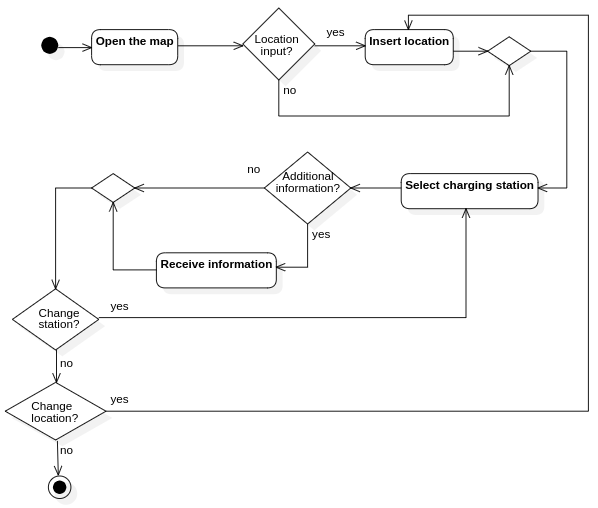
\includegraphics[width=0.9\linewidth]{StateDiagrams/get_charging_stations_location_state_diagram}
    \caption{Get locations of charging stations state diagram}
    \label{fig: locations_sd}
\end{figure}

\textbf{EVD wants to book a charge at a specified charging station at a certain timeframe}

Now, Andrew needs to book a charge for his EV. Ones the choice of the charging station is done, he selects it on the map
and enters the booking section.
If the charging station cannot offer reservation to EVD because of not availability status, the EVD is notified.
Mario has to decide in which timeframe wants the charging point to be reserved.
So, he gets availability schedule of the charging station and selects when he thinks to go to charge.
If it is no more available, the EVD is returned at the previous section.
Otherwise, if there is a caution to pay it is shown to the EVD.
Finally, the EVD receives an e-mail that confirms the reservation, with all the useful information.

It is shown a state diagram that summaries the activities in the booking process:
\begin{figure}[H]
    \centering
    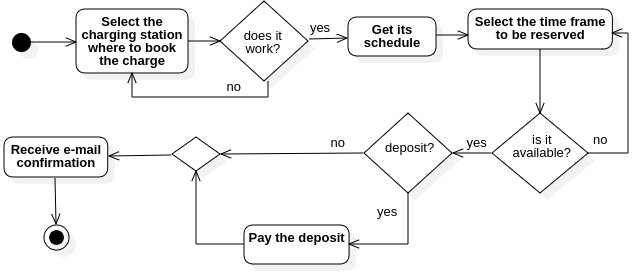
\includegraphics[width=0.9\linewidth]{StateDiagrams/book_a_charge_state_diagram}
    \caption{Book a charge state diagram}
    \label{fig: booking_sd}
\end{figure}

\textbf{CPO wants to add charging points in its CPMS}

\verb|LIGHT| is the new company of the successful businessman Nole Mask.
They decided to trust the \verb|eMALL| project, entrusting them the responsibility of managing their IT infrastructure.
After logging in, they start inserting new charging points owned by them distributed in the territory.
If it belongs to a new charging station, it has to be created too.
So, they insert all the information they are requested (location, costs, connectors, power, etc.).
After they confirm and submit what they inserted, they can add a new charging point.
Otherwise, they easily end the process.

It is shown a state diagram to summaries the activities in the charging points insertion process:
\begin{figure}[H]
    \centering
    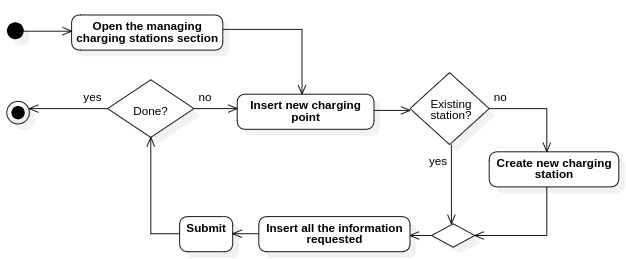
\includegraphics[width=0.9\linewidth]{StateDiagrams/insert_charging_points_state_diagram}
    \caption{Insert charging points state diagram}
    \label{fig: insert_charging_points_sd}
\end{figure}

\section{Product functions}\label{sec:product_functions}


\section{User characteristics}\label{sec:user_characteristics}


\section{Assumptions, dependencies and constraints}\label{sec:assumptions_dependencies_and_constraints}